\chapter{Feature Location Techniques}
%\section{Eins - Eins}
%\subsection{Eins - Eins - Eins}

% Die Logos sind veraltet und duerfen zurzeit nicht verwendet werden!
% Auf Seite \pageref{Logo} in Abbildung \ref{Logo} befindet sich das SE Logo.
In this chapter we want to look at four different feature location techniques in detail. We choose two static and two dynamic techniques with each one technique giving plain and one giving guided output. The techniques presented in the following can be classified by the characteristics of chapter\ref{ch:Classification and Methodology}:

\begin{table}[h]
	\hspace{-3em}
	\begin{tabular}{|l| l l l l l l|}
		\hline
		 & technique &  output & underlying & input & result & user \\ 
		 &  &  &  technology &  &  &  \\ \hline
		 \multirow{5}{1em}{\begin{sideways} static \end{sideways}}
		 & Find-concept  & plain & PDA, NLP & query & AOIG & ++  \\
		 &      &        &             & query         & documents  &   \\
		 & SNIAFL & plain & tf-idf, LSI, & set of query's & BRCG & -/+ \\ 
		 &        &       & PDA  &             &      &
		 \\ 
		 & Dora & guided & PDA, tf-idf & method, depth & call graph & + \\ 
		 &      &        &             & query         & documents  &   \\ \hline
		 \multirow{4}{1em}{\begin{sideways} dynamic \end{sideways}}
		 & Software Reconnaissance  & plain & FCA, PDA & set of & executable & +++ \\ 
		 &   &  &  & scenarios, query & & \\
		 & Revelle  & guided & trace analysis & scenario and & executable, & +\\
		 &   &  & LSI, HITS & query & documents & \\ \hline
		
	\end{tabular}
	\caption{The techniques discussed further on in this paper}
	\label{tab:techniques overview}
\end{table}

\section{Static - Plain}
\label{sec:find-concept}
As an example of a static technique with plain output the \emph{Find-concept (short FC)} of David Shepherd, Emily Hill, K. Vijay-Shanker and Lori Pollock of the University of Delaware and also Martin P. Robillard of the McGill University in Canada is a reasonable choice
The technique makes, as previously mentioned in Chapter \ref{ch:Classification and Methodology}, some assumptions to the underlying code. To apply \emph{FC} the code has to be object-oriented, the comments and identifiers, which are objects and methods, have to be named in a way so that the technique can retrieve domain knowledge. Also it makes the premise that verbs correspond to methods and nouns refer to objects. Also FC defines so called \textit{direct objects}, which are objects corresponding to a verb. In our example the verb $save$ corresponds to $MindMapMapModel$, $MindMapNodeModel$ and $MindMapEdgeModel$, which are therefore the direct objects of $save$.\newline
\emptyLine
The input to the FC is given by the user as a query of description phrases of the feature of interest and after that decomposed into a set of \textit{verb-DO} pairs. In order to improve the result the technique collects related words,like synonyms or verbs in different time forms, and also regards words, which are often mentioned in the context of words from the query. These collected words then get ranked by their similarity to the query words with for example LSI \ref{ch:lsi}, calculating with a variable weight for the synonyms, and the ten most analogous are presented to the user to augment the query with these terms and program methods already matching to the current query.\newline
\emptyLine
The important aspect the user wants to retrieve are the \textit{verb-DO} pairs matching the query. To be able to derive the matching pairs the FC builds an \textit{action-oriented identifier graph model (AOIG)}. The \textit{AOIG} contains four kinds of nodes and 2 types of edges:
%\vspace{3em} %WARNING: may be shitty

\begin{table}[th]
	\begin{tabular}{r l}
		\textit{verb nodes}: & a node for each specific verb/action \\
		\textit{direct object (DO) nodes}: & a node for each direct object \\
		\textit{verb-DO nodes}: & a node for every \textit{verb-Do} pair. (A \textit{DO} can be in multiple \textit{verb-DO} nodes) \\
		\textit{use nodes}: & a node for each incidence of a \textit{verb-DO} pair in comments or the source code \\
		 & \\
		\textit{pairing edges}: & connecting every verb and DO to the \textit{verb-DO nodes} containing them \\
		\textit{use edges}: & connecting each \textit{verb-DO node} to every corresponding \textit{use node}.
	\end{tabular}
\end{table}

After several steps of improving the query the final query traverses through the \textit{AOIG} and filters every \textit{verb-DO} pair containing words of the query, extracting all methods using the filtered pairs and apply \textit{Program Dependency Analysis (PDA)} on it to reveal call relations within the extraction.

Finally the \emph{FC} is able to generate the result graph with methods matching the query as nodes and structural relations between the methods computed by the \textit{PDA}. \cite{shepherd2007using} \newline
Due to the overhead of computing the \textit{verb-DO} pairs out of the query and the step by step improvement of the input the user interaction in Table \ref{tab:techniques overview} is rated with "++".

\section{Static - Guided}
The technique presented by \emph{Emily Hill, Lori Pollock} and \emph{K. Vijay-Shanker}, professors of the \textit{University of Delaware} in  \textit{Computer and Information Science}, is named \emph{Dora the Program Explorer} (short: \emph{Dora}})\footnote{Dora comes from exploradora, the Spanish word for a female explorer\cite{hill2007exploring}. Also the name chosen in account of the children's series "\textit{Dora the Explorer}" }.
Dora also uses a call graph $G=(V,E)$ to derive dependency, like the \emph{Find-concept} in section~\ref{sec:find-concept}, but combines it with the \emph{tf-idf} ranking method explained in section \ref{ch:tf-idf} with the methods as nodes $n \in V$, it's body as the documents $d(n)$ and edges $e=(n,m) \in E$ if $n$ calls $m$. \newline
As an input the user has to yield an initial query, a so called \textit{seed method}$ n_0 \in V$ the examination should start from, and a depth defining a graph-neighbourhood, which should be included in the search(i.e. a maximal distance). \newline
Given the input Dora proceeds by traversing through the call graph $G$ calculating how suitable the document $d(n)$ of the current node $n$ is by combining the succeeding three values:
\begin{enumerate}
	\item the \emph{tf-idf} score of the identifiers within the method name ($n$)
	\item the \emph{tf-idf} score of the identifiers within the method body ($d(n)$)
	\item a binary value to indicate if the method belongs to a library or is part of the user-made code
\end{enumerate}
Dora can be parametrized by the weight of these three components, for example the method name(1) should be more important than the method body(2) and if the method is out of a library it shouldn't be considered, which leads to the following formulae:
\begin{center}
	$\quad s(n)= (1-b) * [ \frac{2}{3} $\emph{tf-idf}$(n) + \frac{1}{3}$\emph{tf-idf}$(d(n)) ]$
\end{center} 
where $b$ defines if $n$ belongs to a library($b=1$) or $n$ is user-made($b=0$).
There are two more adjustable values: the relevance threshold($rt$) and exploration threshold($et$). The relevance threshold determine whether a node is relevant or not can be parametrized by giving a value $rt,et \in [0,1] $ and typically $et < rt$, that given a node $n$:
\vspace{2em} %WARNING: might be shitty
\begin{table}[h]
	\centering
	\begin{tabular}{r c l}
		$rt <= s(n)$ & $\rightarrow$ & the node is relevant\\
		$et <= s(n) < rt$ & $\rightarrow$ & the node isn't relevant, but maybe it's neighbours \\
		$s(n) < et$ & $\rightarrow$ & the node can be neglected
	\end{tabular}
\end{table}

In the case of 1 and 2 Dora traverses to the neighbourhood of the node, if it doesn't harm the the initial depth, and otherwise discards the node. So in finite steps of traversing through the call graph Dora has reached a point, where no additional elements need to be explored.\newline
The result Dora computes is a subgraph $G'=(V',E')$ of the call graph, where $V' = \{ n \in V | et <= s(n) \}$, $E' = \{ (n,m) \in E | n,m \in V' \}$ and a function \newline
\[
	f: n\in V' \rightarrow \{0,1\},n \rightarrow 
		\left\{
			\begin{array}{ll} 
				1, & s(n) >= rt \\
				0, & else 
			\end{array}\right. .
\]
This function can be described as a colouring of every \textit{relevant} node. The final output is the coloured sub-call-graph $G'$. \newline
\emptyLine
In the \textit{Freemind Example} of chapter \ref{ch:Freemind Example} the result can look different, by changing the parameters like the \textit{seed method}, the \textit{depth} or the \textit{threshold values}.
Simplifying the method in the fact of disregarding the method body's and by knowing that every method called in the diagram \ref{dia:freemind callgraph} is user made, the scores are equal to their score in chapter \ref{tab:tfidf_table}. \newline
The threshold are choosen like the following:
\begin{table}[h]
	\centering
	\begin{tabular}{r l}
		$rt = 0.5$ & methods with a score of 0.5 or higher are considered relevant \\
		$et = 0.1$ & methods with a score of 0.3 or higher should be explored further
	\end{tabular}
\end{table}
So the final graph Dora computes looks like the graphfigure \ref{dia:dora result}. The green nodes are relevant to the feature, the grey nodes are explored but not relevant. The red node(\#2) is highly relevant to the feature with a \emph{tf-idf score} of 1.454, but isn't explored due to the \textit{depth} of 3.
\begin{figure}[h]
	\centering
	\begin{tikzpicture}
		\tikzset{vertex/.style = {shape=ellipse,draw,minimum size=1.5em}}
		\tikzset{edge/.style = {->,> = latex'}}
		% vertices
		\node[vertex, fill=black!30!green] (p1) at  (0,2) {\#1};
		\node[vertex, fill=black!30!red] (p2) at  (3,2) {\#2};
		\node[vertex, fill=gray] (p3) at  (0,0) {\#3};
		\node[vertex, fill=gray] (p4) at  (3,0) {\#4};
		\node[vertex, fill=gray] (p5) at (-1,-1)  {\#5};
		\node[vertex, fill=gray] (p6) at (-1,-2.5) {\#6};
		\node[vertex, fill=gray] (p7) at (1,-1)  {\#7};
		\node[vertex, fill=gray] (p8) at (1,-2.5) {\#8};
		%edges
		\draw[edge] (p1)  to (p3);
		\draw[edge] (p4)  to (p2);
		\draw[edge] (p7)  to (p3);
		\draw[edge] (p3)  to (p5);
		\draw[edge] (p5)  to (p6);
		\draw[edge] (p7)  to (p4);
		\draw[edge] (p8)  to (p4);
		\draw[edge] (p8)  to (p7);
	\end{tikzpicture}
	\caption{The result graph of \textit{Dora}, with \#1 as \textit{seed method}, \textit{depth}=3, rt=0.5 and et=0.1}
	\label{dia:dora result}
\end{figure}
 In modern cases of application the \textit{threshold}-values are chosen by a heuristic of other cases and general knowledge of the underlying program. Including the \textit{methods body} (2) and the binary value of the formulae the result can be refined by slightly changing the query or the \textit{threshold's}. \newline
\emph{Dora} only needs a query and a \textit{depth} to compute a result, which takes to further interaction, which is marked within the Table \ref{tab:techniques overview} with only one "+".

\section{Dynamic - Plain}
One of the most important dynamic plain approaches is the very first one of Norman Wilde and Michael Scully known under the term \emph{Software Reconnaissance}. \textit{Software Reconnaissance} tries to define a feature $f$ by getting two sets of scenarios $S_f$ and $\overline{S_f}$ as an input and distinguishing between scenarios that invoke the feature of interest $S$ and scenarios that don't $\overline{S_f}$. \newline
Regarding the execution traces \textit{Software Reconnaissance} categorizes methods/lines of code $M$\footnote{the degree of fineness is chosen by the user} into three groups:
\begin{table}[h]
	\begin{tabular}{l}
		1. potentially involved  \\
 		\qquad $I_1 = \{ m \in M | \exists s \in S_f$ s.t. $s$ executes $m \}$ \\
 		\qquad get executed by \underline{at least one} scenario of $S_f$\\
		2. indispensably involved  \\
		\qquad $I_2 = \{ m \in M | \forall s \in S_f : s$ executes $m \}$ \\
		\qquad get executed by \underline{every} scenario of $S_f$\\
		3. uniquely involved  \\
		\qquad $I_3 = \{ m \in M | m \in I_1$ and $\forall s\in \overline{S_f} : s$ does \underline{not} execute $m \}$ \\
		\qquad executed by at least one scenario of $S_f$ and by no scenario of any other feature\\
		4. common components  \\
		\qquad $C = \{ m \in M | \forall s \in S_f \cup \overline{S_f}:s$ executes $m \}$ \\
		\qquad used by every scenario (for example a \textit{main}-method)
	\end{tabular}
\end{table}
The result are the first 3 lists for every feature $f$ that is set in the query and once the list of all \textit{common} components. Different versions of this technique state, that $I_2 \cap C = \emptyset$.\cite{wilde1995software} \newline
\emptyLine
In our example regarding the two features of $f_1 = automaticSaveFile$ and $f_2 = manualSaveFile$ the execution traces are quite similar owed to the fact, that the \textit{automaticSaveFile}-feature is just a not user triggered \textit{internalSave}. Keeping in mind the callgraph(\autoref{dia:freemind callgraph}) methods \#3, \#5 and \#6 will be considered as \textit{common} components. Method \#1 will be considered \textit{uniquely involved} to the feature $f_1$. \newline
\emptyLine
This technique already requires voluminous overhead, because of the two sets of scenarios $S_f$ and $\overline{S_f}$ for every feature.


\section{Dynamic - Guided}
The dynamic guided technique by Meghan Revelle, Bogdan Dit and Denys Poshyvanyk, which are professors at the College of William and Mary in Virginia, is based on a chain of other techniques here and further named as the main author:
\begin{center}
	$Revelle \rightarrow Liu \rightarrow Poshyvanyk \rightarrow Marcus$
\end{center}
\label{ref:marcus}
The very base technique by Marcus is to take given an input query and convert it into a document in vector space using the in \autoref{ch:lsi} mentioned \textit{LSI}. The technique then separates different software elements, for example methods, and creates separate documents using the identifiers and also converting them into vector space. The identifiers are often separated using typical code style, like the connecting of two words using "\underline{ }" or changing from lower to upper case letters. In order to filter the result the search space in partitioned by refining the documents similarity values, so that in step $i+1$ are only the documents of step $i$, which are higher than a given threshold. After that the user decides which documents are relevant to the feature. Once the user decides that no further document is relevant to the feature the the algorithm terminates. \cite{marcus2004semantic} \newline
%In addition to \textit{Marcus} \textit{Poshyvanyk} uses FCA \autoref{sec:FCA} to rank the documents after they are ranked on the similarity to the input query. \textit{Poshyvanyk} takes the first $n$ documents and ranks the \emph{uniquely} appearing terms in the documents based on the similarity the term and the corpus-document in a way, that terms, which are similar to terms in the $n$ documents but not in the rest, are ranked higher. On the other hand terms, which are similar to documents not being in the top $n$ documents, are penalized because might have identifiers for not relevant things with relevant names and therefore would distort the result. After ranking the unique terms \textit{Poshyvanyk} selects the top $k$ terms as \textit{attributes} out of the top $n$ documents, which are the \textit{objects}, and apply FCA \autoref{sec:FCA}. So the user gets not only the space vectors of the similarity of the documents, but also gets a visualization of the terms used within. \newline
\textit{Poshyvanyk} uses a combination of \textit{Marcus} \textit{LSI} method and \textit{execution-trace analysis} \footnote{further information on that topic within the \textit{IEEE}-paper \cite{antoniol2006feature}}. To analyse a program is has to be given as an input in an executable form, to determine if which methods are called on a scenario, and a set of documents, which can be defines out of a query with \textit{Marcus}. Also the technique needs two sets of scenarios: one that invoke the feature of interest and one that doesn't. First the technique ranks the documents like within \textit{Marcus}. After that the scenario sets are executed and execution profiles are derived. By that the methods can be ranked by the appearance within the traces of the scenarios that execute the feature versus the appearance within the other scenarios. The final result of a method is a weighted sum of the \textit{LSI}-rank and the \textit{trace}-rank. So the final output is the again a ranked list of methods. \cite{poshyvanyk2007feature} \newline
The technique \textit{Liu} is quite similar to \textit{Poshyvanyk}, with the difference, that instead of using two sets of scenarios \textit{Liu} only works with a single scenario executing the feature of interest. This reduces the overhead of input and also accelerates the process, accepting the fact that the result may not be as accurate as it would be with \textit{Poshyvanyk}. \cite{liu2007feature} \newline
The technique \textit{Revelle} combines \textit{Information Retrieval}, \textit{dynamic} and \textit{web-mining} analysis in order to improve the results of the previous methods. Like \textit{Riu} \textit{Revelle} gets a single scenario that exercises the feature of interest and a query as input. While running the scenario the call graph from the execution trace is constructed, which nodes are methods that are actually executed. Every node gets a score using a web-mining algorithm like the HITS-algorithm mentioned in \autoref{sec:HITS}. After assigning the values \textit{Revelle} filters one of the following two out:
\begin{itemize}
	\item low-ranked methods 
	\begin{itemize}
		\item typically used on \textit{HITS authority score}
		\item methods that aren't called often aren't extremely important
	\end{itemize}
	\item high-ranked methods 
	\begin{itemize}
		\item typically used on \textit{HITS hub score}
		\item  methods that call very many other methods aren't meaningful
	\end{itemize}
\end{itemize} 
The remaining set of methods get ranked by using \textit{Liu} and the final ranked list is returned to the user.
The overall user interaction is quite sparely, because of one scenario and a query about the feature of interest and therefore rated with "+" in \autoref{tab:techniques overview}. \cite{revelle2010using}

\section{Future Technique Approaches}
All of the presented techniques are still under research to improve the results accuracy, the runtime and the amount of user interaction. Even if the last point isn't that important in the beginning is can be the most essential due to the possibility of high serialisation. Also the generally preferred technique group is the static one, because of the high amount of pre-computing used to derive scenarios and checking if they invoke the feature and the execution time used to run these.\newline
\textit{W. Zhao, L. Zhang, J. Sun and F. Yang} from the University of Peking in cooperation with \textit{L. Yin} of the Rensselaer Polytechnic Institute are working on an approach of a \textit{static non-interactive} technique by using \textit{Program Dependency Analysis} and \textit{Information Retrieval} technologies.\newline
They define two types of functions of a feature:
\begin{enumerate}
	\item \textit{specific functions}:
	functions only used to implement the feature and not used by any other feature.
	\item \textit{relevant functions}:
	functions involved in the implementation of the feature
\end{enumerate}
The set of \textit{specific features} is indisputable a subset of the set of \textit{ relevant features}.
The presentation of the program within the technique is realized with a so called \textit{Branch-Reserving Call Graph (BRCG)}, which is a a normal call graph expanded with branching and sequential information. These informations can be used to construct pseudo execution traces for a feature. The \textit{BRCG} can be written as $G=(V,E)$ with the nodes $V$ as a function, a branch or a return statement. Loops are defined as two branch statements: one going through the loopbody and one exiting immediately. 

%\begin{figure}[hbt]{0.5*\textwidth}
%	\lstset{language=Java}
%	\lstinputlisting[
%	label=lst:system,
%	caption=An example code for BRCG] {src/listings/BRCG-examplecode.java}
%\end{figure}

\noindent\begin{minipage}{.35\textwidth}
	\lstset{language=Java}
	\lstinputlisting[
		label=lst:code,
		caption=An example code for BRCG] {src/listings/BRCG-examplecode.java}
\end{minipage}\hfill
\begin{minipage}{.55\textwidth}
%	\begin{tikzpicture}
%		\tikzset{method/.style = {shape=circle,draw,minimum size=3em}}
%		\tikzset{decision/.style = {shape=diamond,draw,minimum size=1em, node distance=3em}}
%		\tikzset{sequential/.style = {shape=rectangle,draw,minimum width=4em,,node distance=2.25em}}
%		\tikzset{branch/.style = {shape=ellipse,draw,minimum width=3em,node distance=3em}}
%		\tikzset{edge/.style = {->,> = latex'}}
%		
%		\node[method] (method) at  (5,1) {func};
%		\node[sequential, below of=method](method_sequential) {sequential};
%		
%		\node[method, below left = of method_sequential] (f1) {f1};
%		\node[decision, below = of method_sequential](BS1){BS1};
%		\node[branch, below of=BS1](BS1_branching) {branching};
%		\node[method, below right = of method_sequential] (f6){f6};
%		
%		\node[method, below left = of BS1_branching] (B1) {B1};
%		\node[sequential, below of=B1](B1_sequential) {sequential};
%		\node[method, below right = of BS1_branching] (B2) {B2};
%		\node[sequential, below of=B2](B2_sequential) {sequential};
%		
%		\node[method, below left = of B1_sequential] (f2) {f2};
%		\node[method, below right = of B1_sequential] (exit) {exit};
%		
%		\node[decision, below left = of B2_sequential] (BS2) {BS2};
%		\node[branch, below of=BS2,node distance=3em](BS2_branching) {branching};
%		\node[method, below right = of B2_sequential] (f5) {f5};
%	\end{tikzpicture}

%	\begin{forest}
%		method/.style = {shape=circle,draw,minimum size=3em},
%		decision/.style = {shape=diamond,draw,minimum size=1em},
%		sequential/.style = {shape=rectangle,draw,minimum width=4em,,node distance=2.25em},
%		branch/.style = {shape=ellipse,draw,minimum width=3em,node distance=3em},
%		edge/.style = {->,> = latex'}
%		[{func},method
%			[{f1}, method],
%			[{BS1}, method],
%			[{f6}, method]
%		]
%	\end{forest}
	\vspace{-5em}
	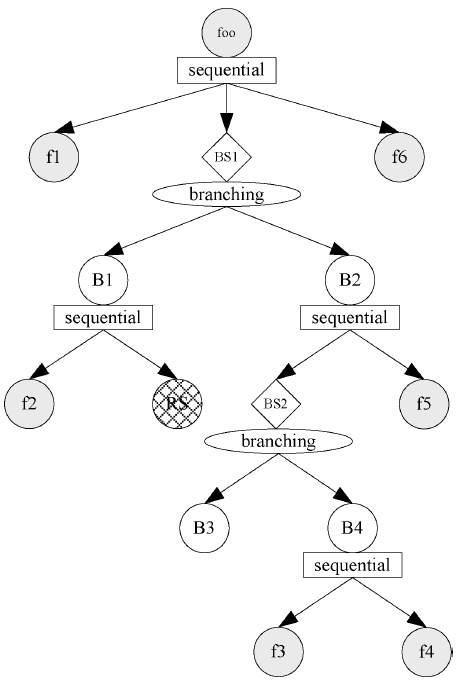
\includegraphics[width=.75\textwidth]{src/pic/BRCG-example.png}
	\captionof{figure}{The BRCG of the example code in \autoref{lst:code} \cite{zhao2006sniafl}}
\end{minipage}


%\clearpage
